\documentclass{beamer}

\usepackage{caption,subcaption}
\usepackage{pgf,tikz}
\usepackage{pgfplots}
\usepackage{tikz-3dplot}
\usetikzlibrary{shapes.geometric,arrows,arrows.meta,decorations.pathreplacing,bending}

\title{Differential Geometry}
\author{Module II}
\institute{Chapter 6 : The Gauss Map}

\begin{document}

\begin{frame}
\maketitle
\end{frame}

\begin{frame}{Gauss Map and Spherical Image}
\begin{block}{Oriented $n$-Surface}
\begin{itemize}
	\item $n$-surface, $S$
	\item Orientation, $\mathbf{N}(p) = (p,N(p))$
\end{itemize}
\end{block}
\begin{definition}[Gauss Map]
	The associated funcion of the smooth, unit normal vector field $\mathbf{N}$ on the $n$-surface $S$ is the \textbf{Gauss Map}, $N : S \to S^n$
\end{definition}

\begin{definition}[Spherical Image]
	The image of the Gauss map $N(S) = \{ q \in S^n : q = N(p),\ p \in S \}$ is the \textbf{spherical image} of the oriented $n$-surface $S$.
\end{definition}
\end{frame}

\begin{frame}{Compact, Connected, Oriented $n$-Surface}
\begin{theorem}[Spherical Image of Oriented $n$-Surface]
\begin{itemize}
	\item Compact, Connected, Oriented $n$-Surface $S$
	\item The Gauss Map $N : S \to S^n$ is surjective.
	\item The Spherical Image is $N(S) = S^n$, unit $n$-sphere.
\end{itemize}
\end{theorem}
\begin{block}{Importance of Compactness}
\begin{itemize}
	\item Counter-example : $n$-Plane $S$
	\item $N(S) = \left\{ \frac{-\nabla f(p)}{\|\nabla f(p) \|} : p \in S \right\}$ is singleton
	\item If oriented $n$-surface $S$ is compact and connected, then\\
		$S$ divides $\mathbb{R}^{n+1}$ into two parts - inside and outside
	\item {\color{green!50!black}Compute the distance of $q \in \mathbb{R}^{n+1}$ from an $n$-surface $S$ ?}
\end{itemize}
\end{block}
\end{frame}

\begin{frame}{Proof : Spherical Image of Oriented $n$-Surface}
\begin{block}{Step 1 : Lagrange multiplier theorem}
\begin{itemize}
	\item $v \in S^n$
	\item $g : \mathbb{R}^{n+1} \to \mathbb{R},\ g(p) = p \cdot v$
	\item Level Sets $g^{-1}(c)$ are $n$-planes parallel to $v^\perp$
	\item By Lagrange multiplier theorem, the restriction of $g$ to $n$-surface $S$ attains maximum and minimum at $p,q$
	\begin{itemize}
		\item $(p,v) = \nabla g(p) = \lambda \nabla f(p) = \lambda \|\nabla f(p) \|\mathbf{N}(p) = (p,\pm v)$
		\item $(q,v) = \nabla g(q) = \lambda \nabla f(q) = \lambda \|\nabla f(q) \|\mathbf{N}(q) = (q,\pm v)$
	\end{itemize}
	\item By intermediate value theorem, if there exists a continuous function $\alpha : [0,1] \to \mathbb{R}^{n+1}$ such that
	\begin{itemize}
		\item $\alpha(0) = p$, $\alpha(1) = q$, $\dot{\alpha}(0) = (p,v)$, $\dot{\alpha}(1) = (q,v)$ 
		\item $\alpha(t) \notin S,\ 0 < t < 1$
	\end{itemize}
	then $N(p) \ne N(q)$
\end{itemize}
\end{block}
\end{frame}

\begin{frame}{Proof : Spherical Image of Oriented $n$-Surface}
\begin{block}{Step 2 : Construction of $\alpha$}
\begin{itemize}
	\item $\exists S_1$ such that $S \subset S_1$ since $S$ is bounded(compact)
	\item $0 < x < y < 1$
	\item $\alpha_1 : [0,x] \to \mathbb{R}^{n+1},\ \alpha_1(t) = p+tv$
	\item $\alpha_2 : [y,1] \to \mathbb{R}^{n+1},\ \alpha_1(t) = q+(t-1)v$
	\item $\alpha_3 : [x,y] \to S_1$ such that
	\begin{itemize}
		\item $\alpha_3(x) = \alpha_1(x) = p+xt$
		\item $\alpha_3(y) = \alpha_2(y) = q+(y-1)v$
	\end{itemize}
\item $$\alpha(t) = \begin{cases} \alpha_1(t) & t \in [0,x)\\ \alpha_3(t) & t \in [x,y] \\ \alpha_2(t) & t \in (y,1] \end{cases}$$
\end{itemize}
\end{block}
\end{frame}

\begin{frame}{Proof : Spherical Image of Oriented $n$-Surface}
\begin{figure}
	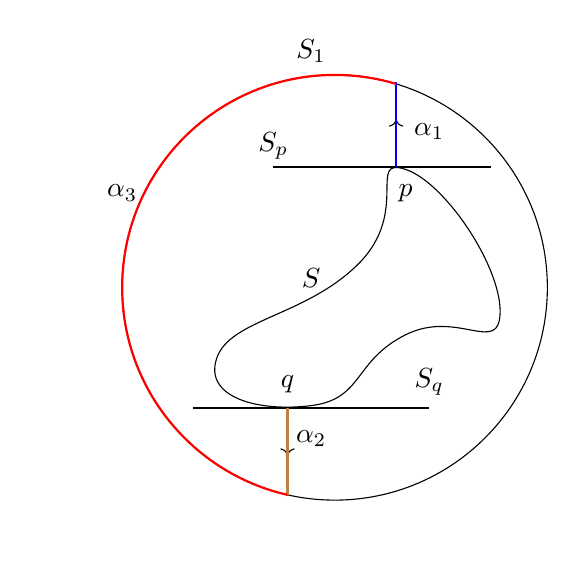
\begin{tikzpicture}[scale=0.6]

	\draw (2,2.5) node{$p$};
	\draw (-0.5,-1.55) node{$q$};
	\draw plot [smooth cycle, tension=1] coordinates {(1,1) (2,3) (4,0) (2,-0.5) (0,-2) (-2,-1)};

	\onslide<1>{
	\draw[->] (1.8,3.05) -- (1.8,4.05);
	\draw (-0.8,3.05) -- (3.8,3.05); %S_p
	\draw (-0.8,3.5) node{$S_p$};

	\draw[->] (-0.5,-2.05) -- (-0.5,-3.05);
	\draw (0.5,0.5) circle (4.5cm);

	\draw (-2.5,-2.05) -- (2.5,-2.05); %S_q
	\draw (2.5,-1.5) node{$S_q$};
	}

	\draw (0,0.7) node{$S$};
	\draw (0,5.5) node{$S_1$};
	\onslide<2>{
	\draw[thick,blue] (1.8,3.05) -- (1.8,4.85);
	\draw (2.5,3.8) node{$\alpha_1$};

	\draw[thick,brown] (-0.5,-2.05) -- (-0.5,-3.9);
	\draw (0,-2.7) node{$\alpha_2$};

	\draw (-4,2.5) node{$\alpha_3$};
	\begin{scope}
		\clip (1.8,0) rectangle (-6,6);
		\draw[thick,color=red] (0.5,0.5) circle (4.5cm);
	\end{scope}
	\begin{scope}
		\clip (-0.5,-5) rectangle (-6,0);
		\draw[thick,color=red] (0.5,0.5) circle (4.5cm);
	\end{scope}
	}
\end{tikzpicture}
	\caption{Construction of $\alpha$}
\end{figure}
\end{frame}

\begin{frame}{Proof : Spherical Image of Oriented $n$-Surface}
\begin{block}{Step 3 : $N(p) \ne N(q)$}
\begin{itemize}
	\item $n$-Surface $S = f^{-1}(c) \implies f(p) = c,\ \forall p \in S$
	\item $f \circ \alpha (0) = c$ and $f \circ \alpha (1) = c$
	\item $(f \circ \alpha)'(0) = v$ and $(f \circ \alpha)'(1) = v$
%		$$(f \circ \alpha)' (0) = \frac{d}{dt}(p+tv) = v$$
%		$$(f \circ \alpha)'(1) = \frac{d}{dt}(q+(t-1)v) =  v$$
	\item {\color{blue}$(f \circ \alpha)'(t) = \nabla f(\alpha(t)) \cdot \dot{\alpha}(t)$} (by Chain Rule)\\
	$(f \circ \alpha)(0) = \|\nabla f(p)\| \mathbf{N}(p) \cdot (p,v) = \| \nabla f(p) \| N(p) \cdot v$\\
	$(f \circ \alpha)(1) = \|\nabla f(q)\| \mathbf{N}(q) \cdot (q,v) = \| \nabla f(q) \| N(q) \cdot v$
\item Suppose $N(p) = N(q)$\\
	$\implies (f \circ \alpha)'(0)$ and $(f \circ \alpha)'(1) $ are of the same sign
	\item Case 1 : $f \circ \alpha$ is increasing at both $0$ and $1$
	\begin{itemize}
		\item For $\epsilon > 0,\ f \circ \alpha(\epsilon) > c$ and $f \circ \alpha (1-\epsilon) < c$
		\item $\exists t$ such that $t \in (0,1)$ and $f \circ \alpha(t) = c$
		\item $\exists t \in (0,1)$ such that $\alpha(t) \in S$ {\color{red} contradicts $\alpha(t) \notin S,t \in (0,1)$}
	\end{itemize}
	\item Case 2 : $f \circ \alpha$ is decreasing at both $0$ and $1$
	\begin{itemize}
		\item For $\epsilon > 0,\ f \circ \alpha(\epsilon) < c$ and $f \circ \alpha (1-\epsilon) > c$
	\end{itemize}
\end{itemize}
\end{block}
\end{frame}

\begin{frame}
	\vspace{0.6in}
	\hspace{3cm} {\color{blue}\Huge{Thank You}}
\end{frame}
\end{document}
